% Asset ID: AS2StatisticalSamplingTIKZ-001
% Unit: AS2 Applied Mathematics
% Topic: AS2-SAMP Statistical sampling
% Purpose: Population, sample, sampling unit and sampling frame diagram
% Source: Supplied Data Collection PDF pages 5-6 and transcript Data Collection 1
% Linked LO IDs: AS2-SAMP-LO001, AS2-SAMP-LO002

\documentclass[tikz,border=8pt]{standalone}
\usetikzlibrary{fit,positioning,arrows.meta,calc}

\begin{document}
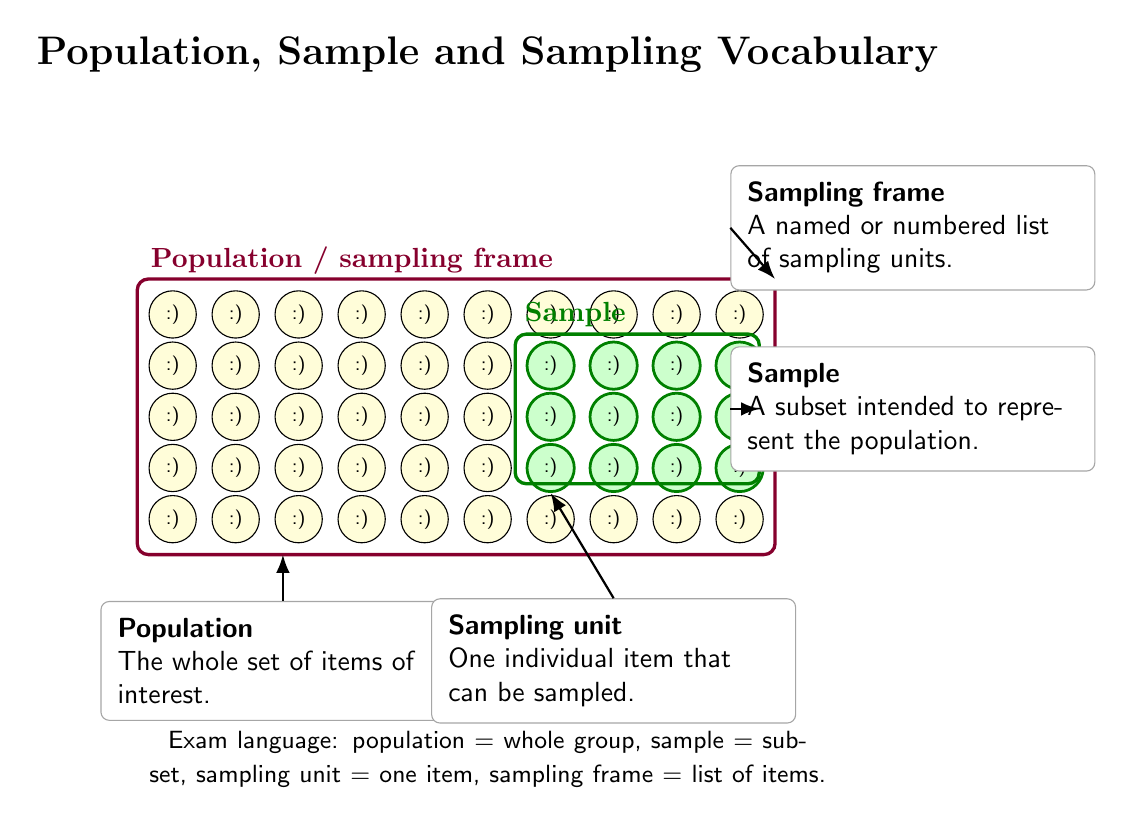
\begin{tikzpicture}[
  font=\sffamily,
  item/.style={circle,draw=black,fill=yellow!15,minimum size=6mm,inner sep=0pt},
  sampleitem/.style={circle,draw=green!50!black,fill=green!20,minimum size=6mm,inner sep=0pt,line width=1pt},
  callout/.style={draw=black!35,fill=white,rounded corners=3pt,text width=4.2cm,align=left,inner sep=6pt},
  arrow/.style={-Latex,thick}
]

\node[font=\bfseries\Large] at (4,5.9) {Population, Sample and Sampling Vocabulary};

\foreach \r in {0,...,4}{
  \foreach \c in {0,...,9}{
    \pgfmathsetmacro{\x}{0.8*\c}
    \pgfmathsetmacro{\y}{0.65*\r}
    \node[item] (u-\r-\c) at (\x,\y) {\scriptsize :)};
  }
}

\foreach \r in {1,2,3}{
  \foreach \c in {6,7,8,9}{
    \pgfmathsetmacro{\x}{0.8*\c}
    \pgfmathsetmacro{\y}{0.65*\r}
    \node[sampleitem] (s-\r-\c) at (\x,\y) {\scriptsize :)};
  }
}

\draw[purple!70!black,line width=1.2pt,rounded corners=4pt] (-0.45,-0.45) rectangle (7.65,3.05);
\node[font=\bfseries,anchor=west,purple!70!black] at (-0.4,3.28) {Population / sampling frame};
\draw[green!50!black,line width=1.2pt,rounded corners=4pt] (4.35,0.45) rectangle (7.45,2.35);
\node[font=\bfseries,anchor=west,green!50!black] at (4.35,2.6) {Sample};

\node[callout] (popdef) at (1.4,-1.8){\textbf{Population}\\The whole set of items of interest.};
\node[callout] (unitdef) at (5.6,-1.8){\textbf{Sampling unit}\\One individual item that can be sampled.};
\node[callout] (sampledef) at (9.4,1.4){\textbf{Sample}\\A subset intended to represent the population.};
\node[callout] (framedef) at (9.4,3.7){\textbf{Sampling frame}\\A named or numbered list of sampling units.};

\draw[arrow] (popdef.north) -- (1.4,-0.45);
\draw[arrow] (unitdef.north) -- (s-1-6.south);
\draw[arrow] (sampledef.west) -- (7.45,1.4);
\draw[arrow] (framedef.west) -- (7.65,3.05);
\node[align=center,text width=11cm] at (4,-3.05){\small Exam language: population = whole group, sample = subset, sampling unit = one item, sampling frame = list of items.};
\end{tikzpicture}
\end{document}
